% ECE501 Digital Image Processing -- End-Semester Report (Group 15)
% Build: tectonic main.tex   (tables are generated by: python End_Sem_Report/make_tables.py, from the repo root)
\documentclass[conference]{IEEEtran}
\usepackage{amsmath,amssymb}
\usepackage{graphicx}
\usepackage{booktabs}
\usepackage{multirow}
\usepackage{array}
\usepackage[hyphens]{url}
\usepackage{cite}

\begin{document}

\title{Fabric Surface Defect Detection and Localization on AFID with Classical Texture Descriptors: from One-Class Texture References to a Supervised Multi-Scale Detector}

\author{\IEEEauthorblockN{Rinal Shah, Varun Hotani, Aadi Mehta, Pratik Agrawal}
\IEEEauthorblockA{ECE501 Digital Image Processing, Group 15}}

\maketitle

\begin{abstract}
We detect and localize defects in woven fabric on the AITEX Fabric Image Database (AFID) using only classical image processing: illumination flattening, median filtering, CLAHE, GLCM, local binary patterns, Gabor filter banks, a per-pixel filter bank and the Hough transform. A first, one-class system modelled defect-free texture per fabric. Under a leak-free protocol it reached only 1.1\,\% pooled pixel IoU, and diagnosis showed why: within a strip its scores barely rank defects above background (AUROC 0.54), because AFID's defect-free and defective images differ globally. The final system keeps the classical descriptors but learns defect appearance from the dataset's masks, with gradient-boosted trees on $16\times16$ windows with strip-normalised, multi-scale context. It is evaluated by 5-fold cross-validation grouped by strip, with every threshold chosen on validation strips. It reaches 0.98 window AUROC, 62.3\,\% patch F1, 80.8\,\% image-level accuracy over 245 strips, and 20.9\,\% pooled pixel IoU (33.9\,\% when the single strip holding 48\,\% of all defect pixels is excluded).
\end{abstract}

\begin{IEEEkeywords}
fabric defect detection, texture analysis, GLCM, local binary patterns, Gabor filters, Mahalanobis distance, gradient boosting, conformal prediction, AFID
\end{IEEEkeywords}

%=====================================================================
\section{Introduction}
Automatic inspection of woven fabric must find defects that are often a few pixels wide on a periodic background whose appearance changes with the weave, the yarn and the illumination. The AITEX Fabric Image Database (AFID) \cite{silvestre2019} provides 245 line-scan strips of $256\times4096$ pixels from seven fabrics: 140 defect-free strips and 106 defective strips with pixel masks for 12 defect classes. This project set out to detect and localize those defects with \emph{classical} digital image processing only: hand-crafted texture descriptors and filter banks, with no learned convolutional features.

The work proceeded in two phases.
\begin{itemize}
  \item \textbf{Phase 1 (one-class, Weeks 3--7).} Per-fabric texture references were fitted on defect-free strips only, and strips were scored by their deviation from them. This phase established the pipeline, the data handling and an honest evaluation protocol. It ended with a diagnosis: within a strip, its scores barely rank defects above background.
  \item \textbf{Phase 2 (supervised, Week 8).} The same descriptors, plus a per-pixel filter bank, train gradient-boosted trees on AFID's masks. Evaluation uses strip-grouped cross-validation, so no test strip ever contributes to training or to any threshold.
\end{itemize}

\emph{Contributions:}
\begin{enumerate}
  \item a reproducible, tested pipeline for AFID, including a complete account of the dataset's quirks
  \item a quantified capture shift between AFID's defect-free and defective images, which bounds any defect-free-only detector
  \item a classical multi-scale detector (window classifier at $16\times16$ with context, pixel filter bank, Hough line linking), evaluated leak-free with precision, recall, F1-score and IoU at pixel, window, patch and image level
\end{enumerate}

%=====================================================================
\section{Related Work}
Gray-level co-occurrence matrices \cite{haralick1973}, local binary patterns \cite{ojala2002} and Gabor filter banks \cite{jain1991,daugman1985} are the standard classical texture descriptors, and all three have been applied to fabric inspection. Novelty detection against a model of normal texture, such as a Mahalanobis distance \cite{mahalanobis1936}, a One-Class SVM \cite{scholkopf2001} or an Isolation Forest \cite{liu2008}, needs defect-free data only. Supervised alternatives need labelled defects; gradient-boosted trees \cite{friedman2001,ke2017} are a strong classical choice for tabular descriptors. The Hough transform \cite{duda1972,matas2000} detects line structures. Conformal prediction \cite{vovk2005} gives distribution-free guarantees on false-alarm rates.

%=====================================================================
\section{Dataset and Evaluation Protocol}
\subsection{AFID}
Strips are $256$ rows (fabric travel) by $4096$ columns (fabric width). Filenames encode \texttt{nnnn\_ddd\_ff}: image, official defect code, fabric code. Five quirks of the published archives are handled explicitly:
\begin{itemize}
  \item a misnamed extra defect-free strip
  \item a defective strip of a non-existent fabric 08 without a mask
  \item two masks split into two files
  \item one empty mask
  \item one $256\times3796$ strip
\end{itemize}
The usable set is 105 defective strips with masks and 140 defect-free strips. Defect classes are highly imbalanced: 39 fuzzy balls, but a single knot, contamination and weft crack.

\subsection{Protocol}
All results use strip-level splits: overlapping windows of one strip never appear on both sides. The one-class phase holds out defect-free strips per fabric (12 fit, 4 calibrate, 4 image-level negatives). The supervised phase uses 5-fold cross-validation grouped by strip and stratified by (defective, fabric). Each outer training fold is split again, by strip, into fit (75\,\%) and validation (25\,\%) strips. Every threshold and configuration choice is made on validation strips by maximising F1, and the test strips are scored exactly once. Metrics are reported \emph{pooled} (TP/FP/FN summed over strips) and as \emph{per-strip means}. Undefined ratios are NaN, not zero.

%=====================================================================
\section{Method}
\subsection{Pre-processing}
Each strip is cropped to the fabric region of interest: columns with mean below 245 and standard deviation above 2, minus a 40\,px selvage margin. It is then illumination-flattened by subtracting a Gaussian blur with $\sigma=50$\,px, median-filtered ($3\times3$) and contrast-normalised with CLAHE (clip 2.0, $8\times8$ tiles).

\subsection{Texture Descriptors}
For square windows at several sizes, the following blocks are computed:
\begin{itemize}
  \item \textbf{GLCM (30-D):} five Haralick statistics at distances 1--3 over four angles (mean and spread across angles), on a min--max stretch quantized to 64 levels.
  \item \textbf{LBP (28-D):} uniform rotation-invariant histograms at $(P,R)=(8,1),(16,2)$.
  \item \textbf{Gabor (24-D):} the mean and standard deviation of magnitude responses of 12 filters ($\lambda=4,8,16$\,px; $0^\circ$--$135^\circ$; one-octave bandwidth).
\end{itemize}
LBP codes and Gabor responses are computed once per strip and pooled per window. All blocks are cached per image and per window size.

\subsection{Phase 1: One-Class Texture References}
Per fabric, a regularised Gaussian model of defect-free $256\times256$ descriptors scores windows by Mahalanobis distance:
\begin{equation}
d_f(\mathbf{x})=\sqrt{(\mathbf{x}-\boldsymbol{\mu}_f)^\top(\boldsymbol{\Sigma}_f+\lambda\tfrac{\operatorname{tr}\boldsymbol{\Sigma}_f}{D}\mathbf{I})^{+}(\mathbf{x}-\boldsymbol{\mu}_f)}.
\end{equation}
The threshold $\tau_f=\mu+k\sigma$ ($k=2.5$) is set on held-out defect-free strips. Flagged windows are refined at $64\times64$ (optionally $32\times32$), and morphology produces the mask. An image-level decision uses a conformal p-value of $\max_i d_f/\tau_f$ against held-out defect-free strips. The ablations compared one-class SVM and Isolation Forest baselines, a pooled \emph{fixed} reference against the per-fabric \emph{adaptive} ones, strip-normalised scoring and an in-domain cross-validated reference.

\subsection{Phase 2: Supervised Multi-Scale Detector}
\emph{Window stage.} Every $16\times16$ window (stride 8) gets a 417-D row with four parts:
\begin{itemize}
  \item its own GLCM, LBP and Gabor blocks
  \item the same blocks robust-$z$-scored within the strip (median/MAD), which cancels strip-wide offsets
  \item the strip-normalised blocks of the nearest $32\times32$, $64\times64$ and $256\times256$ windows (context), found by binary search on the window grid
  \item a fabric one-hot
\end{itemize}
A histogram gradient-boosting classifier \cite{friedman2001,ke2017} (early stopping, at most 1{,}000 rounds) is trained on every defect window and on sampled defect-free windows, with the classes re-weighted. A second classifier on $32\times32$ windows provides an alternative map. Validation selects the $16\times16$ map, the $32\times32$ map or their mean.

\emph{Pixel stage.} Inside candidate windows, each pixel is classified from 30 robust-normalised filter responses:
\begin{itemize}
  \item intensity, and its deviation from 5/15/31\,px medians
  \item local standard deviation over 5, 15 and 31\,px
  \item weft- and warp-line responses: deviation from the column and row medians, smoothed along the yarn over 9 and 33\,px
  \item Laplacian of Gaussian at $\sigma=1,2,4$
  \item smoothed Sobel gradients
  \item the 12 Gabor magnitudes
\end{itemize}

\emph{Line linking.} Probabilistic Hough segments \cite{matas2000} within $10^\circ$ of the yarn directions are redrawn inside flagged windows only, to close gaps in thin detections.

\emph{Decisions.} Validation chooses between the window-map mask and the pixel-stage mask, and sets the gate and pixel thresholds, the Hough settings, and the window, patch and image thresholds, each by maximising F1. Pooled IoU $=F_1/(2-F_1)$ is maximised with it.

%=====================================================================
\section{Results}
\begin{table}[!t]
\centering
\caption{Progression over the project (AFID; \%, except AUROC). Patch F1 and IoU$_\mu$ are per-strip means; pixel F1 and IoU are pooled (TP/FP/FN summed over strips). Image-level AUROC uses 28 (Week~7) or all 140 (final) defect-free strips as negatives.}
\label{tab:progress}
\scriptsize
\setlength{\tabcolsep}{1.6pt}
\begin{tabular}{@{}lrrrrrr@{}}
\toprule
\textbf{System} & $n$ & \textbf{Patch F1} & \textbf{Pix.\ F1} & \textbf{IoU} & \textbf{IoU$_\mu$} & \textbf{AUROC} \\
\midrule
Mid-sem (13 strips) & 13 & 27.1 & -- & -- & 0.4 & -- \\
Week 5 one-class & 105 & 14.0 & 0.7 & 0.3 & 0.3 & 0.675 \\
Week 7 one-class & 105 & 18.4 & 2.2 & 1.1 & 1.4 & 0.790 \\
Supervised (final) & 105 & 58.6 & 34.5 & 20.9 & 14.0 & 0.865 \\
\bottomrule

\end{tabular}
\end{table}

\begin{table}[!t]
\centering
\caption{Final supervised detector: precision, recall, F1 and IoU (\%) at every level (pooled unless stated). $^\dagger$Excluding strip \texttt{0080\_036\_01}, whose mask holds 48\,\% of all defect pixels. $\pm3$\,px: a prediction within 3\,px of a defect pixel counts as correct.}
\label{tab:levels}
\scriptsize
\begin{tabular}{@{}lrrrr@{}}
\toprule
\textbf{Level} & \textbf{Prec.} & \textbf{Rec.} & \textbf{F1} & \textbf{IoU} \\
\midrule
Pixel, pooled & 52.3 & 25.8 & 34.5 & 20.9 \\
Pixel, pooled$^\dagger$ & 52.2 & 49.1 & 50.6 & 33.9 \\
Pixel, $\pm3$\,px & 65.3 & 29.2 & 40.4 & -- \\
Pixel, mean/strip & 28.8 & 40.6 & 21.1 & 14.0 \\
$16^2$ window & 58.0 & 35.0 & 43.7 & 28.0 \\
$32^2$ window & 54.7 & 38.7 & 45.3 & 29.3 \\
$256^2$ patch & 60.3 & 64.3 & 62.3 & 45.2 \\
Image (strip) & 81.5 & 71.4 & 76.1 & -- \\
\bottomrule

\end{tabular}
\end{table}

\begin{table}[!t]
\centering
\caption{Ablation (\%, except AUROC): supervised variants (each a full CV) and one-class systems, including the \emph{fixed} global reference against the \emph{adaptive} per-fabric one.}
\label{tab:ablation}
\scriptsize
\setlength{\tabcolsep}{2.5pt}
\begin{tabular}{@{}>{\raggedright\arraybackslash}p{3.1cm}rrrr@{}}
\toprule
\textbf{Variant} & \textbf{Pix.\ F1} & \textbf{IoU pooled} & \textbf{IoU mean} & \textbf{Img AUROC} \\
\midrule
final: 16x16 +\allowbreak{} 32x32 ensemble, pixel stage, Hough & 34.5 & 20.9 & 14.0 & 0.865 \\
32x32 windows only & 33.4 & 20.1 & 15.1 & 0.872 \\
16x16 +\allowbreak{} 32x32, no pixel stage & 32.4 & 19.3 & 12.1 & 0.865 \\
One-class, per-fabric & 2.2 & 1.1 & 1.4 & 0.790 \\
One-class, global & 0.2 & 0.1 & 0.1 & 0.744 \\
One-class SVM & 2.2 & 1.1 & 1.3 & 0.697 \\
Isolation Forest & 1.8 & 0.9 & 1.0 & 0.669 \\
\bottomrule

\end{tabular}
\end{table}

\begin{table}[!t]
\centering
\caption{Final detector per official defect class (pooled pixel \%, and image-level detection rate).}
\label{tab:defect}
\scriptsize
\setlength{\tabcolsep}{2.5pt}
\begin{tabular}{@{}lrrrrrr@{}}
\toprule
\textbf{Defect} & $n$ & \textbf{Prec.} & \textbf{Rec.} & \textbf{F1} & \textbf{IoU} & \textbf{Det.} \\
\midrule
broken\_end & 9 & 42.1 & 60.3 & 49.6 & 32.9 & 77.8 \\
broken\_pick & 10 & 62.3 & 48.1 & 54.3 & 37.2 & 100.0 \\
broken\_yarn & 8 & 34.3 & 65.6 & 45.0 & 29.1 & 100.0 \\
contamination & 1 & 72.8 & 72.8 & 72.8 & 57.2 & 100.0 \\
crease & 5 & 17.8 & 49.9 & 26.3 & 15.1 & 100.0 \\
cut\_selvage & 9 & 22.7 & 23.0 & 22.9 & 12.9 & 44.4 \\
fuzzy\_ball & 39 & 6.6 & 38.9 & 11.3 & 6.0 & 61.5 \\
knot & 1 & -- & 0.0 & 0.0 & 0.0 & 0.0 \\
nep & 14 & 21.3 & 27.5 & 24.0 & 13.7 & 57.1 \\
warp\_ball & 5 & 7.5 & 33.0 & 12.2 & 6.5 & 80.0 \\
weft\_crack & 1 & 67.3 & 0.6 & 1.2 & 0.6 & 100.0 \\
weft\_curling & 3 & 17.8 & 54.9 & 26.9 & 15.5 & 100.0 \\
\bottomrule

\end{tabular}
\end{table}

\begin{figure*}[!t]
\centering
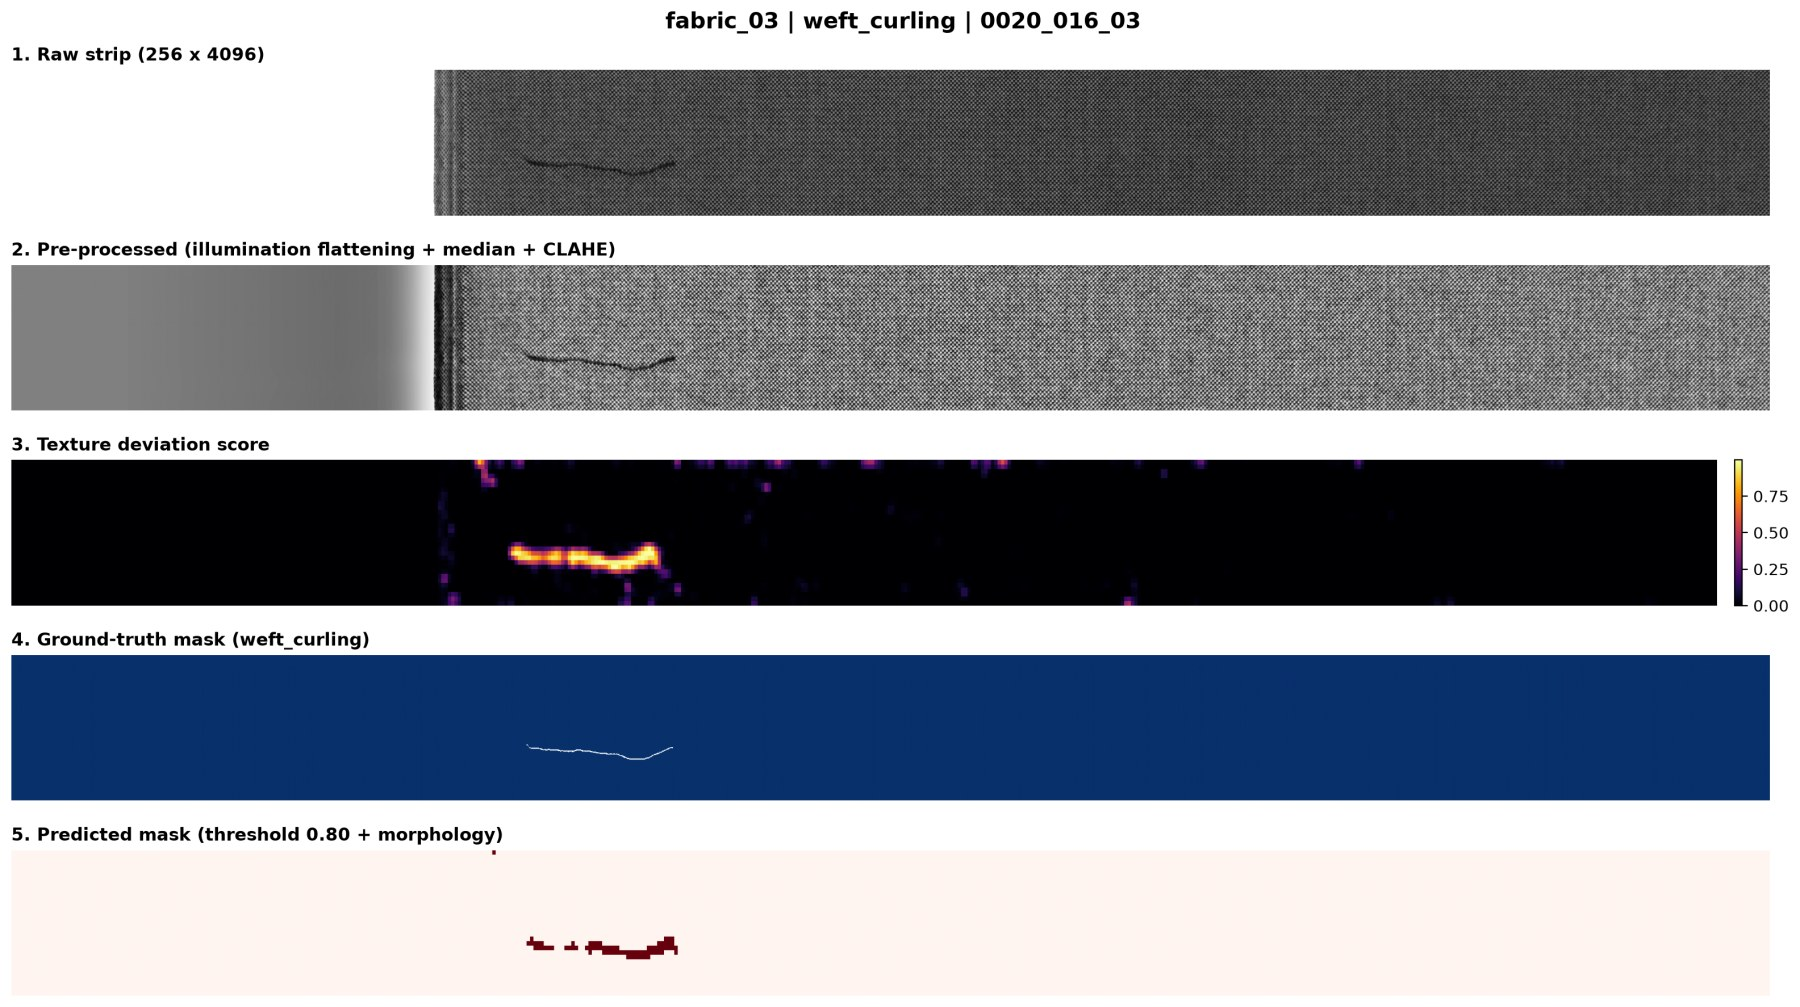
\includegraphics[width=0.49\textwidth]{figures/inspection_0020_016_03.jpg}\hfill
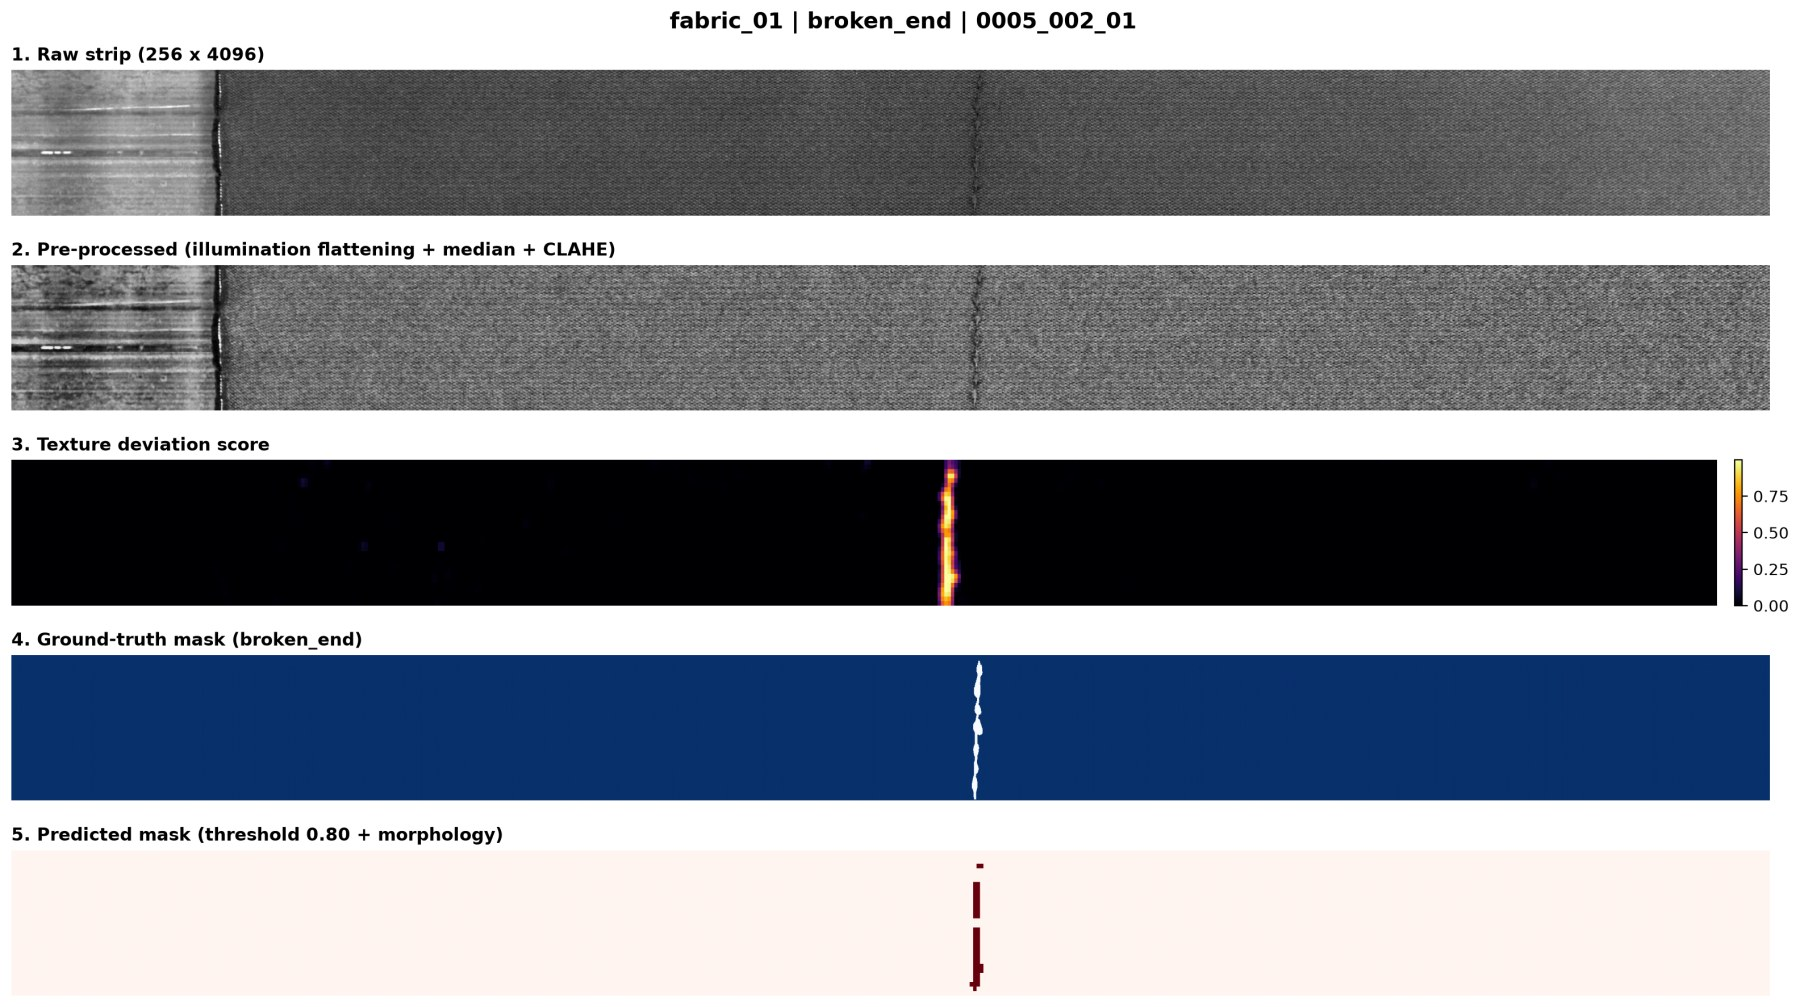
\includegraphics[width=0.49\textwidth]{figures/inspection_0005_002_01.jpg}
\caption{Held-out predictions of the final detector. Left: weft curling (fabric 03). Right: broken end (fabric 01). Panels: raw strip, pre-processed strip, $16\times16$ texture-deviation map, ground truth, predicted mask.}
\label{fig:examples}
\end{figure*}

Table~\ref{tab:progress} traces the project. The one-class system improved between Weeks~5 and~7 but stayed near 1\,\% pooled pixel IoU. The supervised detector, on the same descriptors, reached 20.9\,\%. Table~\ref{tab:levels} gives precision, recall, F1 and IoU at every level:
\begin{itemize}
  \item $16\times16$ windows: AUROC 0.980, F1 43.7\,\%
  \item $256\times256$ patches: F1 62.3\,\%
  \item image level: accuracy 80.8\,\% (75 of 105 defective strips found, 17 false alarms in 140 defect-free strips), F1 76.1\,\%
\end{itemize}
On fabric 03, whose two capture sets match best, image accuracy is 88.2\,\% and image F1 90.3\,\%. Validation selected the $16\times16$ map in 4 of 5 folds (the 16/32 mean in one), the pixel stage in 2 and Hough linking in 3. In the ablation (Table~\ref{tab:ablation}), removing the pixel stage lowers pooled pixel F1 from 34.5 to 32.4\,\%, and $32\times32$-only windows reach 33.4\,\%. Fig.~\ref{fig:examples} shows two held-out strips.

%=====================================================================
\section{Discussion}
\emph{Adaptive vs.\ fixed.} Among one-class systems, per-fabric (adaptive) references beat a single pooled (fixed) reference by a wide margin (Table~\ref{tab:ablation}: 2.2 vs.\ 0.2\,\% pooled pixel F1). In the supervised detector, adaptivity takes the form of within-strip normalisation and a fabric code.

\emph{Capture shift.} Normal windows of defective strips scored far above held-out defect-free strips for five fabrics, so no defect-free-only model could set a threshold that worked on both \cite{quinonero2009}. Strip-normalised features and defect labels remove that obstacle.

\emph{Limitations.}
\begin{itemize}
  \item \textbf{Pooled pixel metrics are dominated by one strip.} The weft crack \texttt{0080\_036\_01} holds 48\,\% of all defect pixels. It is detected at image level, but only 0.6\,\% of its pixels are recovered.
  \item \textbf{Thin defects are delineated a few pixels off.} F1 rises from 34.5 to 40.4\,\% within $\pm3$\,px.
  \item \textbf{Small blobs are found but not outlined.} Fuzzy balls (39 strips) have window AUROC 0.97 but 6\,\% pixel IoU.
  \item \textbf{Several classes have a single example.} Fabric 05 has one defective strip, so per-class results there are anecdotal.
  \item \textbf{Supervision requires pixel masks for training.}
\end{itemize}

%=====================================================================
\section{Conclusion}
Classical texture descriptors are sufficient to \emph{find} fabric defects on AFID, provided the decision is learned from labelled defects rather than from defect-free data alone. Evaluated without leakage, a gradient-boosted detector on $16\times16$ GLCM, LBP and Gabor windows with strip-normalised multi-scale context reaches 0.98 window AUROC, 62\,\% patch F1 and 81\,\% image accuracy. Exact pixel delineation of thin and small defects (21--34\,\% pooled IoU) is the main remaining limitation.

\bibliographystyle{IEEEtran}
\bibliography{references}

\end{document}
